\chapter[Geothermal Refrigeration]{Geothermal Refrigeration}

For the goal of real cooling and providing thermal comfort to the population, it is necessary to follow the Laws of Nature, specifically transferring thermal energy from an environment to a colder thermal reservoir. In practice, outer space is the only cold source when analyzing planetary thermodynamics. The interior of planets has high temperatures due to the effect of gravitational pressure \cite{Simon–Glatzel}, and we receive thermal energy from the Sun during the day - part of which is retained in the atmosphere by the Greenhouse Effect. However, since the planet continuously loses thermal energy to space, there is always a cold source underground (\autoref{soil-temp}). In other words, at a certain depth in the soil, the temperature tends to be lower than at the surface during the day.

\begin{table}[h]
\centering
\ABNTEXfontereduzida
\caption{Soil Temperature vs Depth}
\legend{Fonte: https://renouvelable-habitat.fr/en/soil-temperature-at-2m-depth}
\label{soil-temp}
\begin{tabular}{ccc}
\hline
Depth(m)  &    Temperature(°C)\\
\hline
0.5 & 10 – 15 \\
1 & 12 – 15 \\
2 & 13 – 16 \\
3 & 14 – 16 \\
4 & 15 – 17 \\
5 & 15 – 18 \\
10 & 18 – 25 \\
300 & 25 – 30 \\
1000 & 30 – 50 \\
\hline
\end{tabular}
\end{table}

Geothermal refrigeration is naturally more efficient than an air conditioner because it follows the natural flow of heat. There are various ways to design a geothermal refrigerator, but the principle of all is the same: bury some fluid a few meters below the ground and use a pumping system connected to some thermal radiator. Using water as a fluid is the most natural option due to its excellent thermal capacity and the fact that it is abundant on Earth.

The temperature of the soil varies according to the latitude on the planet, type of soil, season of the year, and time of day, among many other factors. Therefore, the depth of the wells for geothermal refrigeration is a data that must be obtained experimentally, and I cannot estimate in this thesis the amount of heat that can be extracted from the environment using this technology.

However, another advantage of geothermal refrigeration, compared to air conditioners, is the fact that it can be used outdoors. Since this technology truly has the power to cool an environment - by following the natural flow of heat - the effect of its use is beneficial throughout the neighborhood. Unlike air conditioners, which worsen the thermal quality in neighboring spaces.

It is common knowledge that trees positively affect the local climate, cooling it down, and in many cases, making the thermal sensation feel a few degrees lower than in the same city in a less green area. However, this difference is often attributed to the fact that trees provide shade, rather than the main reason, which is that they can draw water stored underground at a temperature much lower than that of the atmosphere at the moment. The goal of geothermal refrigeration is to create the same cooling effect that tree cover generates, but without having to wait for the tree to grow. In addition to the fact that many environments that need cooling cannot have trees on site..

In order to calculate the planetary thermodynamics, it is necessary to divide between organic and inorganic because living beings have their own metabolism that influences the global climate. And life is not distributed equally across the planet; there is much more metabolism within the Amazon than compared to the Sahara Desert.
Similarly, thermal machines are not evenly distributed across the planet; urban centers like São Paulo have much more machinery using energy than a village in Africa. All these parameters still need to be studied in more depth, and it should also be kept in mind that there is a barrier of winds between the Earth's hemispheres, and therefore distinct measures may be necessary between them.

The most usual construction of geothermal refrigerators consists of burying pipes with water or other refrigerant fluids, as shown in (\autoref{geothermal-default}). However, I believe this is an inefficient project compared to creating impermeable wells connected to a pumping system that will create an "urban circulatory system," as shown in (\autoref{geothermal-new}). The reason is simple: the less earth you need to remove for construction, the cheaper it becomes, and the amount of water stored determines the cooling power of that geothermal refrigerator. This is a closed system, meaning that the water added to the well will not leave the system except in case of leaks and damage.
The well is then connected by pipes to multiple thermal radiators so that heat can be exchanged with the environment.

\begin{figure}[ht]
    \centering
    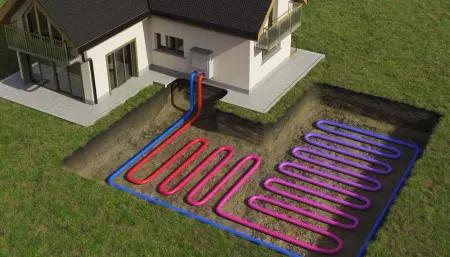
\includegraphics[scale=0.7]{pictures/geoterma-padrao.jpeg}
    \caption{Scheme of a geothermal refrigerator with pipes buried in the ground}
    \label{geothermal-default}
    \legend{Fonte: https://pt.solar-energia.net/energia-renovavel/energia-geotermica, accessed on June 2025}
\end{figure}

\begin{figure}[ht]
    \centering
    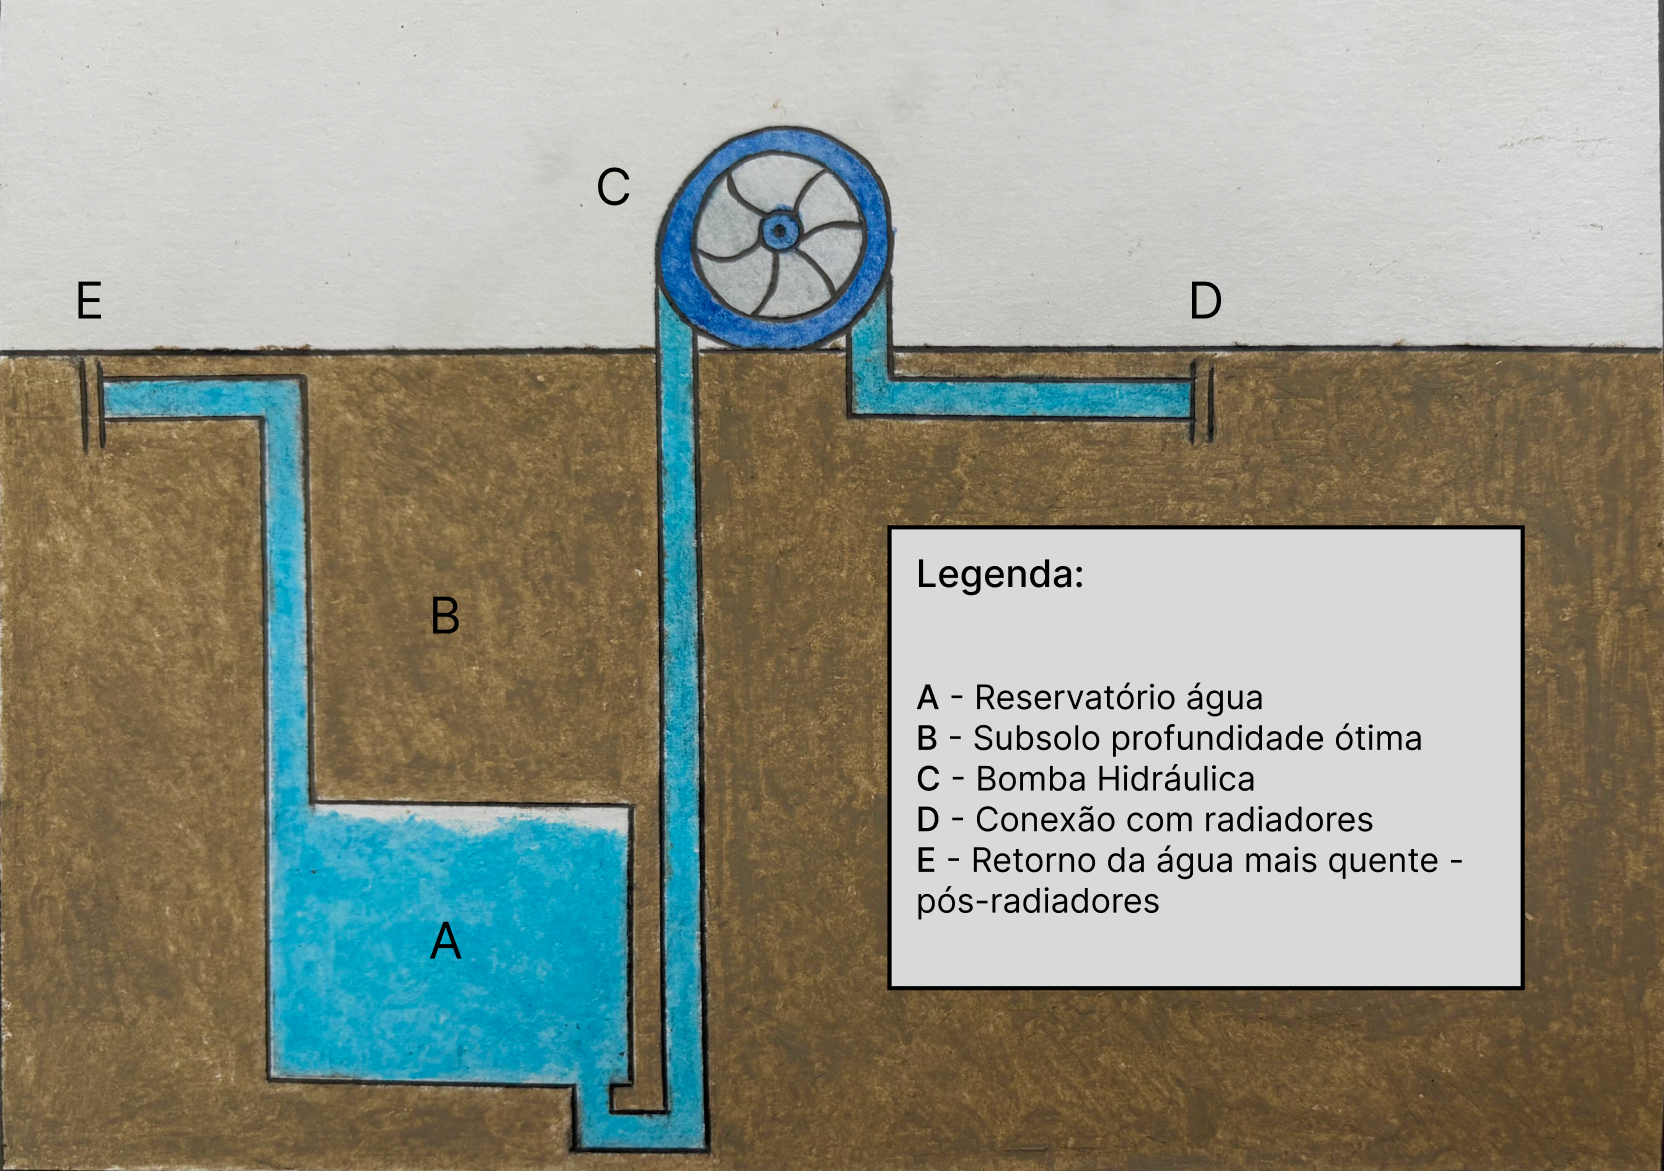
\includegraphics[scale=0.25]{pictures/geoterma.png}
    \caption{Suggestion of a geothermal refrigerator with wells and radiators}
    \label{geothermal-new}
\end{figure}

This technology is not only beneficial for urban centers, as it has the potential to revolutionize agriculture. In addition to being able to create greenhouses with controlled climate, it is possible to combat desertification through the production of organic matter and seedling cultivation. Therefore, geothermal refrigeration greenhouses act in multiple ways against desertification and can be the key to converting unproductive lands into economically autonomous regions. However, for use in closed environments, it may be necessary to use fans attached to the radiators for better efficiency in thermal exchanges. In (\autoref{poste}), I exemplify an outdoor radiator use, and in (\autoref{estufa}), it is an example for a closed environment.

\begin{figure}[ht]
    \centering
    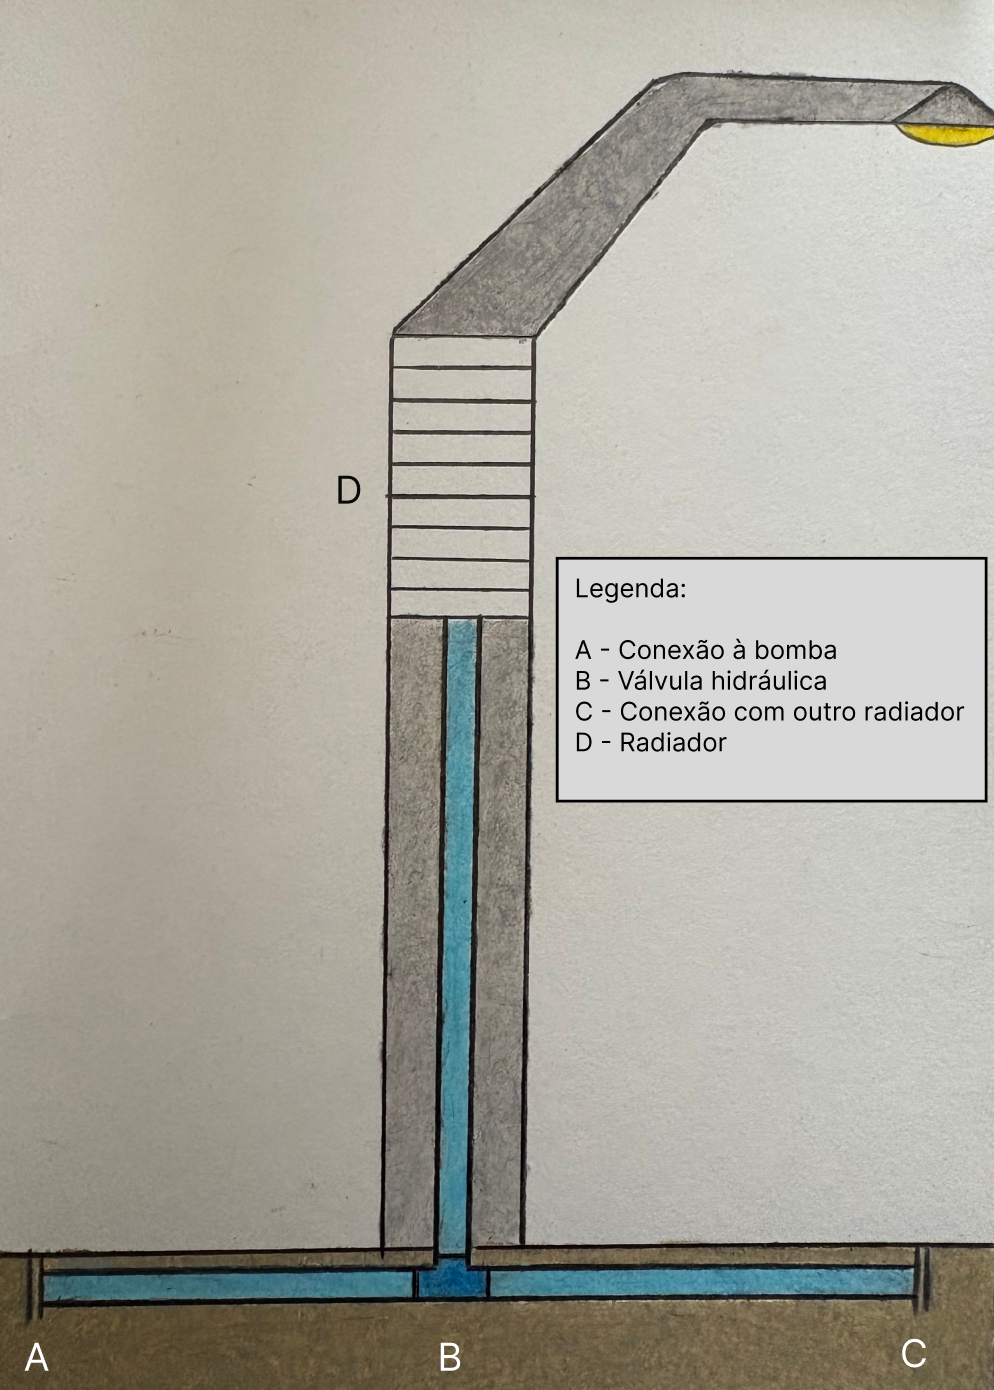
\includegraphics[scale=0.25]{pictures/poste.png}
    \caption{Scheme of construction of an outdoor radiator - ex. street lamp}
    \label{poste}
\end{figure}

\begin{figure}[ht]
    \centering
    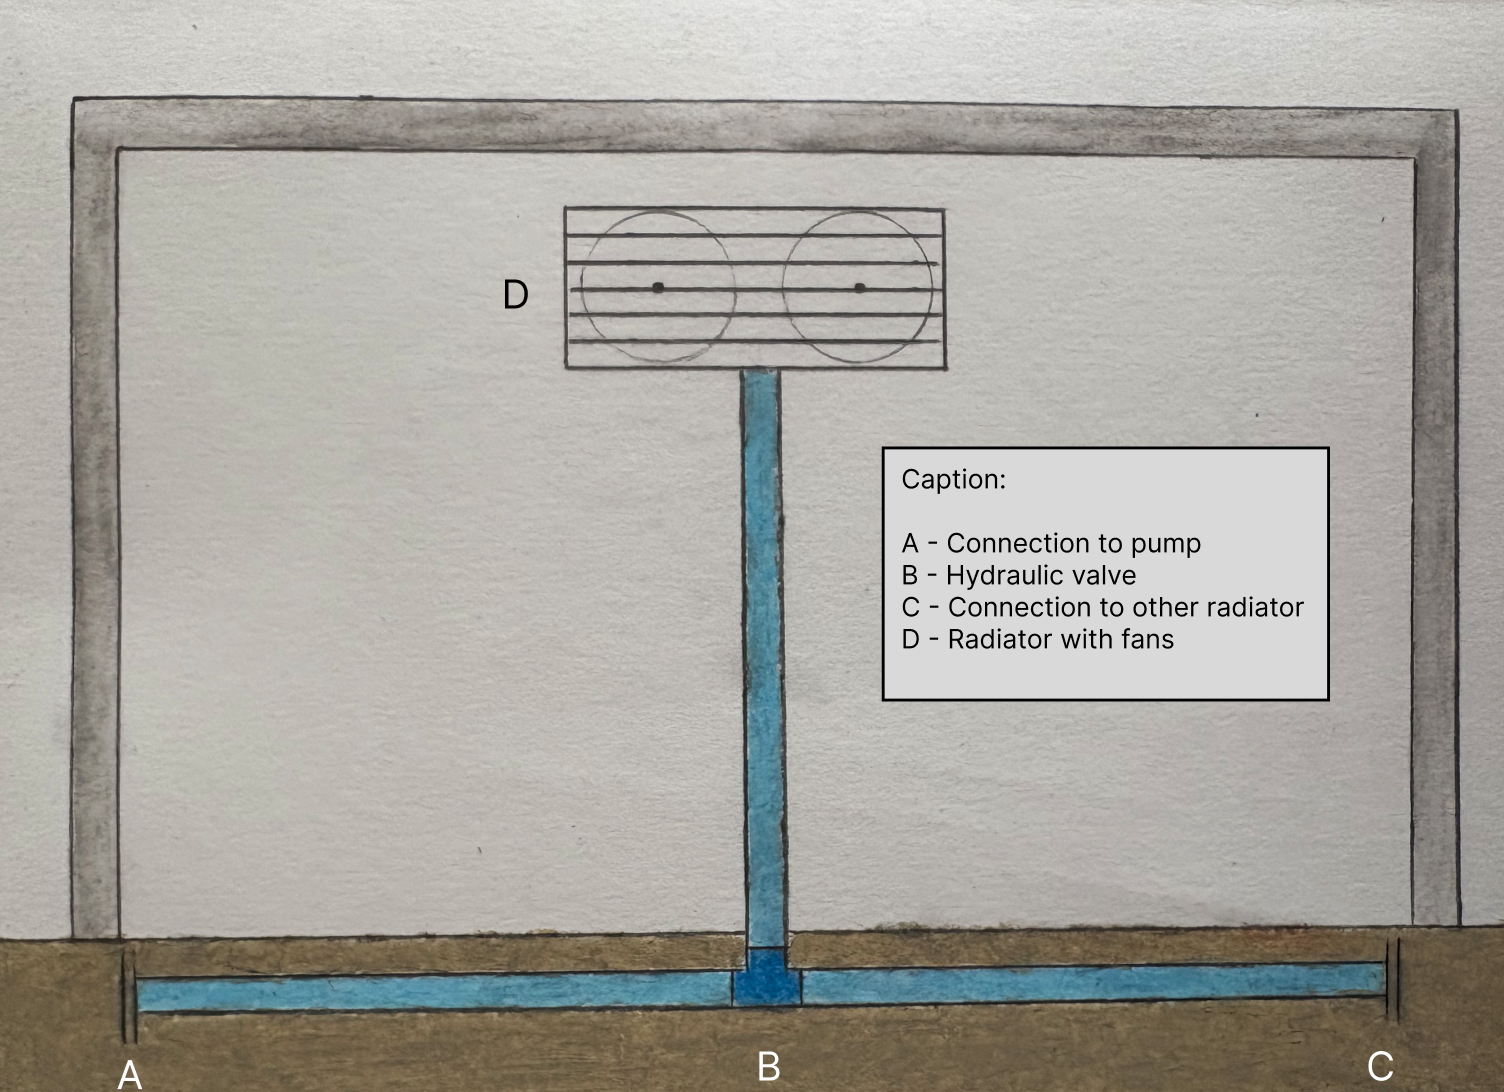
\includegraphics[scale=0.25]{pictures/estufa.png}
    \caption{Scheme of construction of an indoor radiator - ex. greenhouse}
    \label{estufa}
\end{figure}

\section{Experiment}

This thesis is written in a purely theoretical form, and it is necessary to create an experiment to confirm it, always making it clear that scientific development must be empirical and collaborative. The proposed experiment is to choose a metropolitan region with high air conditioner usage and create the first geothermal refrigerator in the area. Once the refrigerator is operational, it is necessary not to use air conditioners and utilize meteorological monitoring systems to verify if the cooling effect aligns with the theory. It is important to remember that it is still not possible to predict how many systems will need to be built to stabilize the Earth's atmosphere, even if this theory proves valid.

As previously mentioned, the ideal depth for the wells - which should be around 2m - varies depending on various factors such as latitude, season of the year, and type of soil. However, since the amount of heat generated in urban areas would decrease with the end of air conditioners, another beneficial effect is that this would be reflected in the temperature of the underground over time, meaning that this system becomes more efficient at removing heat as the years go by.